\begin{tehtavasivu}

% tässä ei käytetä konsistenssin vuoksi euromerkkiä \euro (textmode), vaan sanallista ilmaisua ''euro''

% FIXME: tehtävä: ilmaise desimaalilukuna seuraavat prosentit

% FIXME: tehtävä perusarvosta

% FIXME: laaja tehtävä ansio- ja pääomatulojen verotuksesta

% FIXME: korolle korkoa -laskut esitellään seuraavassa kappaleessa, onko tämä tehtävä tarkoituksella tässä? 
%\begin{tehtava}
%    Erään pankin myöntämä opintolaina kasvaa korkoa $2~\%$ vuodessa. Kuinka monta 
%    prosenttia laina on kasvanut korkoa alkuperäiseen verrattuna kymmenen vuoden kuluttua?
%    \begin{vastaus}
%        $22~\%$.
%    \end{vastaus}
%\end{tehtava}

% FIXME: nykyisessä kappalejärjestyksessä verrannollisuus tulee vasta myöhemmin 
%\begin{tehtava}
%    Kappaleen putoamisen kesto maahan korkeudelta $x$ on kääntäen verrannollinen
%    putoamiskiihtyvyyden $g$ neliöjuureen. Vakio $g$ on kullekin taivaankappaleelle ominainen
%    ja eri puolilla taivaankappaletta likimain sama. Empire State Buildingin katolta (korkeus $381$ metriä)
%    pudotetulla kuulalla kestää noin $6,2$ sekuntia osua maahan. Marsin putoamiskiihtyvyys on $37,6\%$
%    Maan putoamiskiihtyvyydestä. 
%    
%    Jos Empire State Building sijaitsisi Marsissa, kuinka kauan kuluisi kuulan maahan osumiseen?
%    \begin{vastaus}
%        Noin $10$ sekuntia.
%    \end{vastaus}
%\end{tehtava}

\begin{tehtava}
    Oppikirjamaraton-tiimi kävi lounastamassa. Osoita oheisen kuitin tiedoilla vääräksi yleinen virhekäsitys,
    että $13~\%$ arvonlisävero olisi $13~\%$ lopullisesta myyntihinnasta.
    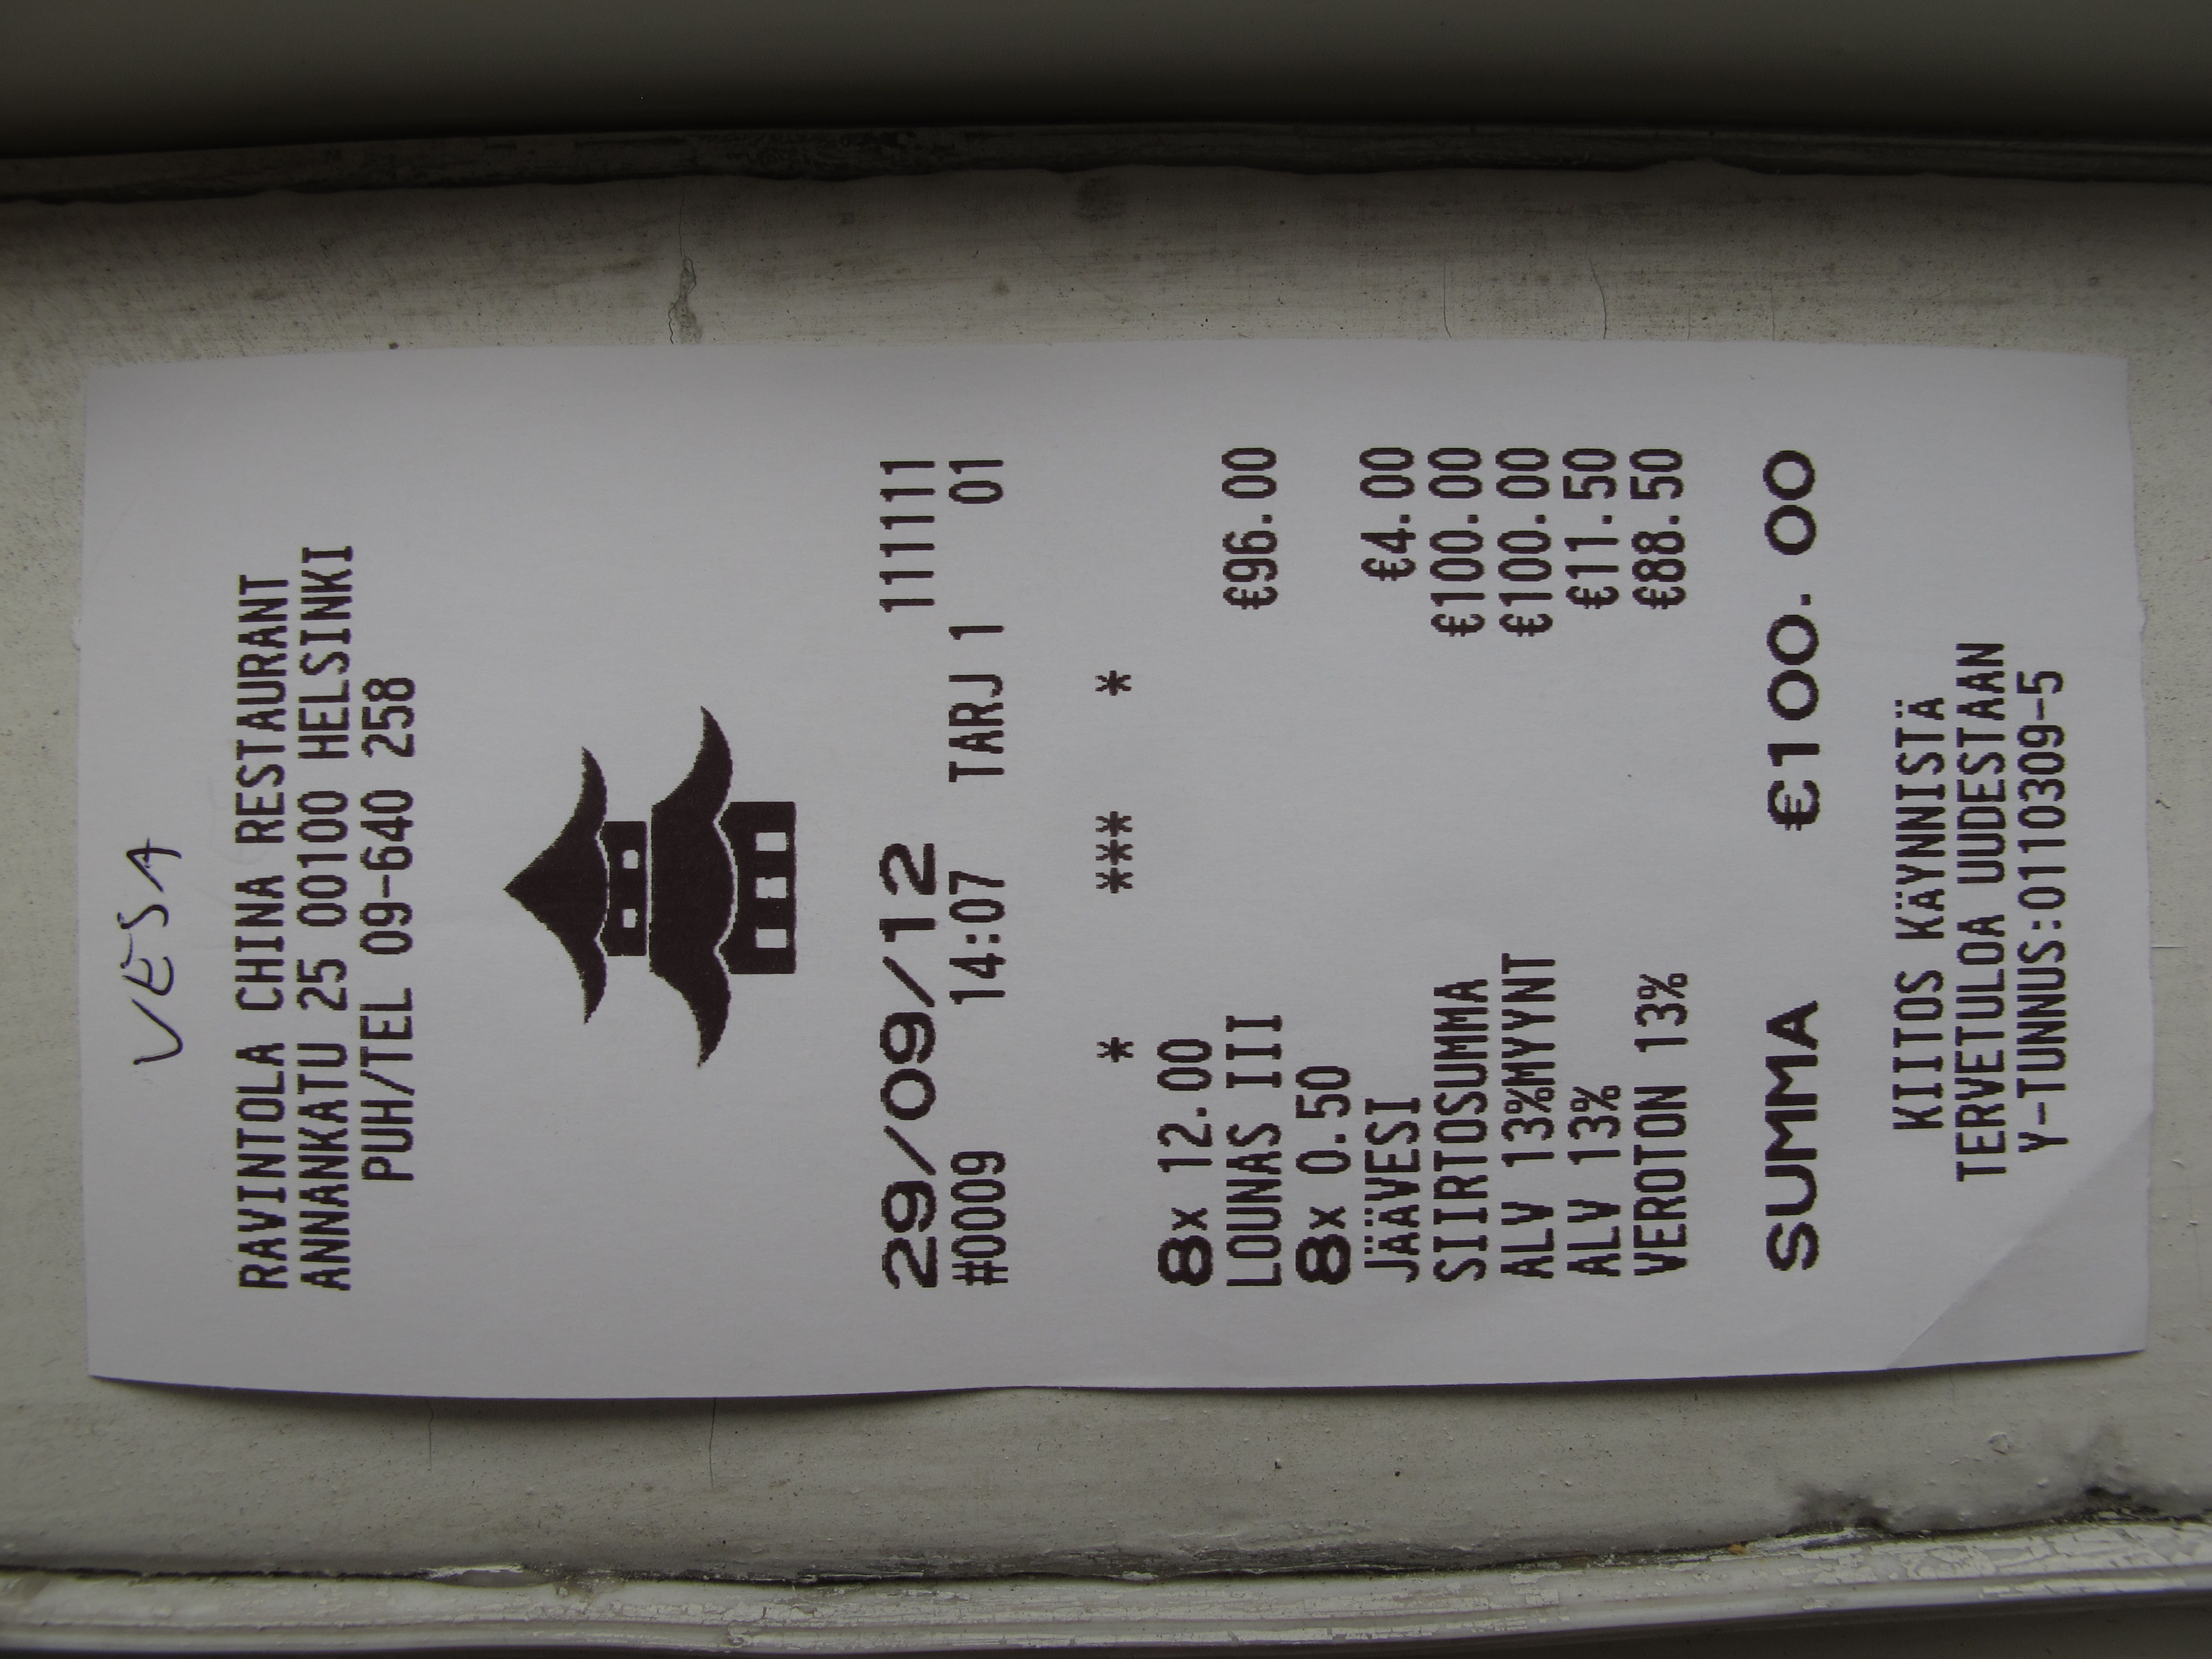
\includegraphics[width=80mm, angle=270]{pictures/alv-kuitti}
    \begin{vastaus}
         $13~\%$ sadasta eurosta on $13$ euroa, ei $11,50$ euroa, niin kuin kuitissa todetaan. Arvonlisävero
         lasketaan suhteessa verottomaan hintaan, ei lopulliseen myyntihintaan.
    \end{vastaus}
\end{tehtava}

\begin{tehtava}
    Laukun normaalihinta on $225$ euroa, ja se on $25$ prosentin alennuksessa.
    Mikä on alennettu hinta?
    \begin{vastaus}
        $168,75$ euroa
    \end{vastaus}
\end{tehtava}

\begin{tehtava}
    Jaakon kuukausipalkka on $1623,52$ euroa. Hän saa $1,3~\%$ palkankorotuksen.
    Mikä on Jaakon kuukausipalkka korotuksen jälkeen?
    \begin{vastaus}
        $1644,63$ euroa
    \end{vastaus}
\end{tehtava}

\begin{tehtava}
    Kirjan myyntihinta, joka sisältää arvolisäveron, on $9~\%$ suurempi kuin kirjan veroton hinta.
    Laske kirjan veroton hinta, kun myyntihinta on $27$ euroa.
    \begin{vastaus}
        Kirjan veroton hinta on $24,77$ euroa.
    \end{vastaus}
\end{tehtava}

\begin{tehtava}
    Sokerijuurikkaassa on $18~\%$ sokeria. Kuinka paljon sokerijuurikkaita tarvitaan valmistettaessa
    $8$ tonnia sokeriliuosta, jonka sokeripitoisuus on $4,5~\%$?
    \begin{vastaus}
        $2$ tonnia
    \end{vastaus}
\end{tehtava}

\begin{tehtava}
    Perussuomalaisten kannatus oli vuoden 2007 eduskuntavaaleissa $4,1~\%$ ja 
    vuoden 2011 eduskuntavaaleissa $19,1~\%$. Kuinka monta prosenttiyksikköä 
    kannatus nousi? Kuinka monta prosenttia kannatus nousi?
    \begin{vastaus}
        Kannatus nousi $15$ prosenttiyksikköä, ja toisaalta $366$ prosenttia.
        Mediassa kannatusmuutokset ilmoitetaan prosenttiyksiköissä.
    \end{vastaus}
\end{tehtava}

\begin{tehtava}
    Askartelukaupassa on alennusviikot, ja kaikki tavarat myydään $60~\%$:n 
    alennuksella. Viimeisenä päivänä kaikista hinnoista annetaan vielä 
    lisäalennus, joka lasketaan aiemmin alennetusta hinnasta. Minkä suuruinen 
    lisäalennus tulee antaa, jos lopullisen kokonaisalennuksen halutaan olevan $80~\%$?
    \begin{vastaus}
        $50~\%$
    \end{vastaus}
\end{tehtava}

\begin{tehtava}
    Hedelmissä on vettä aluksi 60~\%. Kuinka monta prosenttia vedestä on 
    haihdutettava, jotta hedelmissä tämän jälkeen olisi vain 20~\% vettä?
    \begin{vastaus}
        $50~\%$
    \end{vastaus}
\end{tehtava}


\begin{tehtava}
    Samulin pituus on $165$~cm ja Joonaksen $173$~cm.
    \begin{alakohdat}
        \alakohta{Kuinka monta prosenttia Samulin pituus on Joonaksen pituudesta?}
        \alakohta{Kuinka monta prosenttia Samuli on lyhyempi kuin Joonas?}
        \alakohta{Kuinka monta prosenttia Joonas on pidempi kuin Samuli?}
    \end{alakohdat}
    \begin{vastaus}
        \begin{alakohdat}
            \alakohta{$95,4~\%$}
            \alakohta{$4,62~\%$}
            \alakohta{$4,85~\%$}
        \end{alakohdat}
    \end{vastaus}
\end{tehtava}

\begin{tehtava}
    Yleinen arvonlisäveroprosentti oli Suomessa vuonna 2012 $23~\%$ tuotteen
    verottomasta hinnasta. Tuotteen hinta koostuu sen verottomasta hinnasta 
    ja tuotteesta maksettavasta arvonlisäverosta. Kuinka monta 
    prosenttia arvonlisävero on tuotteen myyntihinnasta?
    \begin{vastaus}
        $18,7~\%$
    \end{vastaus}
\end{tehtava}

\begin{tehtava}
    Kun matkalipun hintaa korotettiin $10,0~\%$, matkustajien määrä väheni $10,0~\%$.
    Kuinka monella prosentilla tällöin lisääntyivät tai vähentyivät liikennöitsijän 
    lipputulot?
    \begin{vastaus}
        Vähentyivät $1$ prosentilla.
    \end{vastaus}
\end{tehtava}

\begin{tehtava}
    Tuoreissa omenissa on vettä $80~\%$ ja sokeria $4~\%$. Kuinka monta prosenttia sokeria
    on samoissa omenissa, kun ne on kuivattu siten, että kosteusprosentti on $20$? [K2000, 4]
    \begin{vastaus}
        $16~\%$
    \end{vastaus}
\end{tehtava}

\begin{tehtava}
    Matin ja Iidan duo saa julkisuutta, ja he alkavat myydä CD-levyään keikkojen yhteydessä $10$ euron
    kappalehinnalla. Jonkin ajan päästä he päättävät laskea CD-levyn hintaa $20$ prosenttia. Matti alkaa
    kuitenkin katua päätöstä, ja ehdottaa tämän alennetun hinnan korottamista $20$ prosentilla. Mikä olisi
    tämän toimenpiteen jälkeen CD:n uusi hinta? Montako prosenttia olisi korotuksen oltava, jotta oikeasti
    päästäisiin takaisin alkuperäiseen $10$ euron hintaan?
    \begin{vastaus}
        $25~\%$
    \end{vastaus}
\end{tehtava}

\begin{tehtava}
    Jalkapalloilija Georgios Samaras teki ensimmäisellä kaudellaan Skotlannin valioliigassa (2007-08)
    $5$ maalia Celtic F.C.:n paidassa. Seuraavalla kaudella Samaras teki Celticille liigassa $15$ maalia.
    Kuinka monta prosenttia Samaraksen maalimäärä nousi?
    \begin{vastaus}
        $200~\%$
    \end{vastaus}
\end{tehtava}

\begin{tehtava}
    Kaupungissa tuli jokaisen talonomistajan suorittaa kaupungin kassaan $5~\%$ saadusta
    hyyrymäärästä (vuokrasta, ruotsin sanasta \textit{hyra}). Sittemmin määrättiin, että mainittu
    prosentti oli oleva 10. Monellako prosentilla täytyy talonomistajien korottaa hyyryjä
    saadakseen saman puhtaan säästön kuin ennen? [YO 1877, 4]
    \begin{vastaus}
        $5,6~\%$
    \end{vastaus}
\end{tehtava}

\end{tehtavasivu}
